\documentclass[11pt,a4paper]{book}
\usepackage[utf8]{inputenc}
\usepackage[english]{babel}
\usepackage{amsmath}
\usepackage{amsfonts}
\usepackage{amssymb}
\usepackage{graphicx}
\usepackage{dsfont}
\usepackage[left=2.5cm,right=2.5cm,top=2.5cm,bottom=2.5cm]{geometry}
\title{Solid State Physics}
\linespread{1.2}
\begin{document}
\maketitle
\chapter{Crystal Structure}
\section{Direct lattice}

\vspace*{0.5cm}
\begin{center}
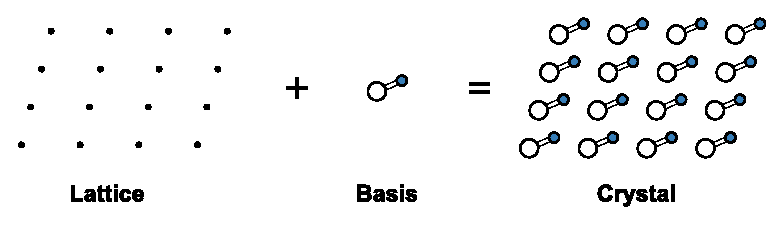
\includegraphics[width=0.75\textwidth]{crystal_structure/figures/crystal.eps}
\end{center}

\noindent
The mathematical description of the crystal consists of two parts: the \emph{lattice} which is a periodic grid of points extending over space and the \emph{basis} which in this context is the set of ions repeating at every lattice point.

The lattice can be described by the set of so called \emph{lattice vectors} $\lbrace\mathbf{R}\rbrace$ given by
\begin{equation}\label{eq:direct_lattice}
\mathbf{R} \equiv \mathbf{R}_{n_1 n_2 n_3}  = n_1 \mathbf{a}_1 + n_2 \mathbf{a}_2 + n_3 \mathbf{a}_3,
\end{equation}
where $n_i \in \mathds{Z}$ and $\mathbf{a}_i$ are linearly independent vectors in the real space called the \emph{primitive vectors}. The primitive vectors have the dimensions of length owing to which the lattice spanned by them is referred to as the \emph{direct lattice}. It should be noted the choice of the primitive vectors is not unique; any non-collinear set of the lattice vectors can be used.

The lattice can be infinite or finite depending on the allowed values of $n_i$. Quite often it is convenient to deal with infinite lattice which extends over all spatial dimensions. In such case the lattice is known as the \emph{Bravais lattice}. 

An important concept of \emph{unit cell} builds upon the lattice. A unit cell is a volume of space that can fill the entire space without overlaps or leaving gaps behind when translated by a suitable set of Bravais lattice vectors. A \emph{primitive unit cell} is a special set of unit cells which enclose precisely one lattice point. Therefore, if the number density of lattice points is $n$, the primitive unit cell volume $v$ is 
\begin{equation}
v = \frac{1}{n}
\end{equation}
regardless the shape of the cell. Sometimes it is, however, easier to work with a \emph{conventional unit cell} instead. For example, a primitive unit cells of a BCC (body-centered cubic) lattice can be difficult to work with since their angles are not orthogonal. The usual choice is to use a cubical cell containing two lattice points instead. Note that whereas primitive unit cells can be translated by all the lattice vectors without any overlaps, the same is not true for the conventional ones. 

There is, however, a common used way to choose a primitive unit cell that has the full symmetry of the lattice. Consider a single lattice point and take all the points in its vicinity that are nearer to it than any other point in the lattice. The volume covered by those points leads to a unique primitive unit cell which is known as the \emph{Wigner-Seitz cell}. The concept is worth remembering as it has an important role in the subsequent discussion.

\vspace*{0.5cm}
\begin{figure}[h!]
\centering
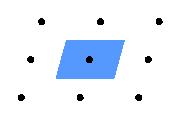
\includegraphics[width=0.4\textwidth]{crystal_structure/figures/wigner-seitz.eps}
\caption{Wigner-Seitz cell of an oblique 2D-lattice. The blue area covers the points closest to the lattice point in the center.}
\end{figure}

\section{Reciprocal Lattice}
In the scope of this for a general plane wave in terms of position $\mathbf{r}$ and time $t$ is written as
\begin{equation}
f(\mathbf{r},t) = A e^{i\mathbf{k}\cdot\mathbf{r} - i\omega t}.
\end{equation}
The wavevector $\mathbf{k}$ points at the direction of propagation of the wave with the length of $k \equiv |\mathbf{k}| = 2\pi/\lambda$, where $\lambda$ is the wavelength. The \emph{angular frequency} (often just frequency) $\omega$ is related to $k$ by $\omega = v k$, where $v$ is the \emph{phase velocity} of the wave.

Dropping out the time-dependent part of the phase $e^{-i\omega t}$, consider a plane wave $e^{i\mathbf{k}\cdot\mathbf{r}}$ with respect to the direct lattice vectors $\mathbf{R}$ defined by Eq.~\eqref{eq:direct_lattice}. In order for the wave to have exactly the same periodicity as the lattice, it needs to have the same value at every single lattice point. This condition can be written as
\begin{equation}
e^{i\mathbf{k}\cdot\mathbf{R}} = 1 \qquad \mathrm{or} \qquad  \mathbf{k}\cdot\mathbf{R} = 2 \pi n, \quad n \in \mathbb{Z}
\end{equation}
for all $\mathbf{R}$. The infinite set of wavevectors $\mathbf{k}$ which fulfil the condition, defines the so-called \emph{reciprocal lattice} which is an extremely useful concept in solid state physics which we shall see in the subsequent chapters. The reciprocal lattice vectors are usually denoted by $\mathbf{G}$.\footnote{Some sources use $\mathbf{h}$ instead.}

Given the primitive vectors $\mathbf{a}_i$ of the direct lattice, any reciprocal lattice can be written as
\begin{equation}
\mathbf{G} \equiv \mathbf{G}_{hkl}  = h \mathbf{b}_1 + k \mathbf{b}_2 + l \mathbf{b}_3,
\end{equation}
where $h,k,l \in \mathds{Z}$ and the reciprocal primitive vectors $\mathbf{b_i}$ are
\begin{equation}
\mathbf{b}_1 = 2 \pi \frac{\mathbf{a}_2 \times \mathbf{a}_3}{\mathbf{a}_1 \cdot \mathbf{a}_2 \times \mathbf{a}_3} \qquad
\mathbf{b}_2 = 2 \pi \frac{\mathbf{a}_3 \times \mathbf{a}_1}{\mathbf{a}_1 \cdot \mathbf{a}_2 \times \mathbf{a}_3} \qquad
\mathbf{b}_3 = 2 \pi \frac{\mathbf{a}_1 \times \mathbf{a}_2}{\mathbf{a}_1 \cdot \mathbf{a}_2 \times \mathbf{a}_3}.
\end{equation}
Thus we see that the set of all $\mathbf{G}$ itself forms a Braivais lattice in the \emph{reciprocal space} (with linear dimensions measured in units of inverse length).

The reciprocal lattice can be also understood from an alternative viewpoint. We may describe the direct lattice in terms of the Dirac delta function as follows:
\begin{equation}
\rho_R(\mathbf{r}) = \sum_{\mathbf{R}} \delta(\mathbf{r}-\mathbf{R}), 
\end{equation}
where the sum goes over all lattice vectors. Therefore $\rho_R(\mathbf{r})$ is function whose value is an (integrable) infinity at the lattice points and zero elsewhere. 
%Now, since the delta function can be presented as
%\begin{equation}
%\delta(\mathbf{r}-\mathbf{R}) = \frac{1}{(2\pi)^3} \int d\mathbf{k} \ e^{i\mathbf{k}\cdot (\mathbf{r}-\mathbf{R})}
%\end{equation}
%we obtain by taking the Fourier transform
Now taking the Fourier transform\footnote{In this document, the convention is that 
$$
\mathcal{F}[f](\mathbf{k})  =  \int d \mathbf{r}\ f(\mathbf{r}) e^{-i\mathbf{k}\cdot \mathbf{r}} \qquad
\mathcal{F}^{-1}[F](\mathbf{r})  = \frac{1}{(2\pi)^3} \int d \mathbf{k} \ F(\mathbf{k}) e^{i\mathbf{k}\cdot \mathbf{r}}
$$} of the lattice we obtain
\begin{equation}
\mathcal{F}[\rho_R](\mathbf{k}) = 
 \sum_{\mathbf{R}} \int d \mathbf{r}\ \delta(\mathbf{r}-\mathbf{R}) e^{-i\mathbf{k}\cdot \mathbf{r}} = \sum_{\mathbf{R}}
 e^{-i\mathbf{k}\cdot \mathbf{R}}.
\end{equation}
The result can be interpreted as the Fourier expansion of a function periodic in terms of $\mathbf{k}$. Since the coefficient is constant for each term, we see that the series is that of the Dirac delta, which is repeated at every $\mathbf{k}$ which fulfils $e^{i\mathbf{k}\cdot\mathbf{R}} = 1$. Thus in terms of the reciprocal lattice vectors $\mathbf{G}$, we may write
\begin{equation}
\mathcal{F}[\rho_R](\mathbf{k}) = (2\pi)^3 \sum_{\mathbf{G}} \delta(\mathbf{k} - \mathbf{G}),
\end{equation}
where the factor of $(2\pi)^3$ comes from the normalisation. Therefore we have shown that the reciprocal lattice can be obtained from the direct lattice \emph{via} the Fourier transform and \emph{vice versa}. This exactly the same procedure how one makes the conversion between the momentum and position in quantum mechanics. We'll see later how the reciprocal space and momentum are related, but it is already now useful to keep in mind, that the reciprocal space is basically just the momentum space in suitable units.

%\begin{equation}
%\mathcal{F}[\rho_R](\mathbf{k}) = \frac{1}{\sqrt{2\pi}^{3}}
% \sum_{\mathbf{R}} \int d \mathbf{r}\ \left[ \frac{1}{(2\pi)^3} \int %d\mathbf{k}' \ e^{i\mathbf{k}'\cdot (\mathbf{r}-\mathbf{R})} \right] e^{-i\mathbf{k}\cdot \mathbf{r}} 
%\end{equation}
%By changing the integration order and reordering the terms, we get
%\begin{equation}
%\mathcal{F}[\rho_R](\mathbf{k}) = \frac{1}{\sqrt{2\pi}^{3}}
% \sum_{\mathbf{R}} \int d \mathbf{k}'\ \left[ \frac{1}{(2\pi)^3} \int d\mathbf{r} \ e^{i(\mathbf{k}'-\mathbf{k})\cdot \mathbf{r}} \right] e^{-i\mathbf{k}\cdot \mathbf{R}} 
%\end{equation}


%\bibliographystyle{plain}
%\bibliography{magnetism/refs}
 
\chapter{Diffraction of X-rays}
\section{Elastic Scattering}

Consider an atom subject to a (classical) electromagnetic magnetic wave whose electric part is given by $\mathbf{E}_0 \cos (\mathbf{k}\cdot\mathbf{r}- \omega t)$. However, since the Maxwell equations and classical mechanics do not mix the real and imaginary parts, we may for mathematical convenience work with the complex exponential plane wave 
\begin{equation}\label{eq:complex_E_wave}
\mathbf{E}(\mathbf{r},t) = \mathbf{E}_0 e^{i \mathbf{k}\cdot\mathbf{r}-i \omega t},
\end{equation}
from which the physical field is recovered by taking its real part. Neglecting the effect of the magnetic field, the Lorentz force affecting an miniscule charge $dq$ is
\begin{equation}
d\mathbf{F} = dq \ \mathbf{E}.
\end{equation}
Substituting the force from Newton's II law $\mathbf{F} = m \ddot{\mathbf{r}} \Rightarrow d\mathbf{F} = dm \ddot{\mathbf{r}}$, we obtain
\begin{equation}\label{eq:charge_acceleration}
\ddot{\mathbf{r}} = \frac{dq}{dm} \mathbf{E}.
\end{equation}
Since the nucleus of the atom is orders of magnitude more massive than electron, we may ignore its movement and thus contribution to the scattering. Thus $dq/dm = -e/m$, where $e$ is the elementary charge and $m$ is the electron mass. Therefore by substituting the wavefield~\eqref{eq:complex_E_wave} to Eq.~\eqref{eq:charge_acceleration}, we get
\begin{equation}
\ddot{\mathbf{r}} = -\frac{e}{m} \mathbf{E}_0 e^{i \mathbf{k}\cdot\mathbf{r}-i \omega t}
\end{equation}
Integrating once with respect to time, we find that the velocity of an infititesimal charge $dq$ intially at rest is
\begin{equation}
\dot{\mathbf{r}} = -\frac{ie}{m\omega} \mathbf{E}_0 e^{i \mathbf{k}\cdot\mathbf{r}-i \omega t}.
\end{equation}
Therefore the current density $\mathbf{J}$ owing to oscillating electons becomes
\begin{equation}\label{eq:oscillating_J}
\mathbf{J}(\mathbf{r},t) = -en(\mathbf{r})\dot{\mathbf{r}} =
\frac{ie^2}{m\omega} n(\mathbf{r}) \mathbf{E}_0 e^{i \mathbf{k}\cdot\mathbf{r}-i \omega t}
\end{equation}
where $n(\mathbf{r})$ is the number density of electrons without the influence of external wavefield.

What kind of wavefield does the oscillating charge density emit? For that we need to solve the 
%wave equations for the scalar potential $\varphi$ and 
wave equation for the vector potential $\mathbf{A}$:
%\begin{align}
%\nabla^2 \varphi - \frac{1}{c^2}\frac{\partial^2 \varphi}{\partial t^2} &= -\frac{\rho}{\varepsilon_0} \\
%\nabla^2 \mathbf{A} - \frac{1}{c^2}\frac{\partial^2 \mathbf{A}}{\partial t^2} &= -\mu_0 \mathbf{J}
%\end{align}
\begin{equation}\label{eq:wave_function_A}
\nabla^2 \mathbf{A} - \frac{1}{c^2}\frac{\partial^2 \mathbf{A}}{\partial t^2} = -\mu_0 \mathbf{J}
\end{equation}
Since the $\nabla^2 - c^{-2} \partial^2_t$ is a linear operator, we seek the solution using the \emph{Green's function}. The Green's function $G(\mathbf{r},t;\mathbf{r}',t')$ is the solution to the problem 
\begin{equation}
\nabla^2  G(\mathbf{r},t;\mathbf{r}',t') - \frac{1}{c^2}\frac{\partial^2 G(\mathbf{r},t;\mathbf{r}',t')}{\partial t^2} = - \delta(\mathbf{r}-\mathbf{r}')
\delta(t-t').
\end{equation}
The solution to the inhomogeneous problem \eqref{eq:wave_function_A} is then
\begin{equation}
\mathbf{A}(\mathbf{r},t) = \mu_0 \int d\mathbf{r}' dt' \   \mathbf{J}(\mathbf{r}',t') G(\mathbf{r},t;\mathbf{r}',t').
\end{equation}
Since the retarded Green's function describing the solutions propagating away from the source is 
\begin{equation}
G(\mathbf{r},t;\mathbf{r}',t') = \frac{1}{4 \pi} \frac{\delta(t'-t_r)}{|\mathbf{r}-\mathbf{r}'|},
\end{equation}
where the retarded time $t_r = t - |\mathbf{r}-\mathbf{r}'|/c$ takes into account the finite speed of light, 
%the solutions to the wave equations are 
the formal solution to the wave equation is 
%\begin{align}
%\varphi &= \frac{1}{4 \pi \varepsilon_0}\int d\mathbf{r}' dt' \  \frac{\rho(\mathbf{r}',t')}{|\mathbf{r}-\mathbf{r}'|} \delta(t'-t_r) \\
%\mathbf{A} &= \frac{\mu_0}{4 \pi}\int d\mathbf{r}' dt' \  \frac{\mathbf{J}(\mathbf{r}',t')}{|\mathbf{r}-\mathbf{r}'|} \delta(t'-t_r).\label{eq:oscillating_A}
%\end{align}
\begin{equation}
\mathbf{A} = \frac{\mu_0}{4 \pi}\int d\mathbf{r}' dt' \  \frac{\mathbf{J}(\mathbf{r}',t')}{|\mathbf{r}-\mathbf{r}'|} \delta(t'-t_r).\label{eq:oscillating_A}
\end{equation}
%Since the atom is electrically neutral, the negative charge of the electron cloud is canceled by the positive nucleus. Sufficiently far away from the atom $\rho(\mathbf{r}',t')/|\mathbf{r}-\mathbf{r}'| \approx 0$, meaning that the scalar potential $\varphi$ vanishes. We are thus left only with a non-zero $\mathbf{A}$. 
Substituting $\mathbf{J}$ fom Eq.~\eqref{eq:oscillating_J} to Eq.~\eqref{eq:oscillating_A}, we get
\begin{align}
\mathbf{A} &= \frac{\mu_0}{4 \pi} \frac{ie^2}{m\omega} \mathbf{E}_0 \int d\mathbf{r}' dt' \  \frac{\delta(t'-t_r)}{|\mathbf{r}-\mathbf{r}'|} n(\mathbf{r}') e^{i \mathbf{k}\cdot\mathbf{r}'-i \omega t'} \nonumber \\ &= \frac{\mu_0}{4 \pi} \frac{ie^2}{m\omega} \mathbf{E}_0 \int d\mathbf{r}' \  \frac{n(\mathbf{r}')}{|\mathbf{r}-\mathbf{r}'|}  e^{i \mathbf{k}\cdot\mathbf{r}'-i \omega t_r}
\end{align}
Considering distances considerably larger than atomic dimensions, we may approximate $|\mathbf{r}-\mathbf{r}'|^{-1} \approx r^{-1}$. In addition, by substituting $t_r = t - |\mathbf{r}-\mathbf{r}'|/c$, we find
\begin{align}
\mathbf{A} &= \frac{\mu_0}{4 \pi} \frac{ie^2}{m\omega}\frac{1}{r} \mathbf{E}_0  \int d\mathbf{r}' \  n(\mathbf{r}')  e^{i \mathbf{k}\cdot\mathbf{r}'+i \omega |\mathbf{r}-\mathbf{r}'|/c -i \omega t} \nonumber \\ &= \frac{\mu_0}{4 \pi} \frac{ie^2}{m\omega}\frac{1}{r} \mathbf{E}_0  e^{-i \omega t} \int d\mathbf{r}' \  n(\mathbf{r}')  e^{i \mathbf{k}\cdot\mathbf{r}'+i k |\mathbf{r}-\mathbf{r}'|},
\end{align}
where in the last step $k=\omega/c$ has been used. By denoting the outgoing wavevector by $\mathbf{k}'$, we recognize that
\begin{equation}
k|\mathbf{r}-\mathbf{r}'| = \mathbf{k}'\cdot(\mathbf{r}-\mathbf{r}') 
\end{equation}
In principle, the direction of $\mathbf{k}'$ depends on $\mathbf{r}'$ but far away from the atom we can regard it being constant. Thus
\begin{equation}
\mathbf{A} = \frac{\mu_0}{4 \pi} \frac{ie^2}{m\omega}\frac{1}{r} \mathbf{E}_0  e^{i \mathbf{k}'\cdot\mathbf{r}-i \omega t} \int d\mathbf{r}' \  n(\mathbf{r}')  e^{i (\mathbf{k}-\mathbf{k}')\cdot\mathbf{r}'}.
\end{equation}

Since we haven't calculated the scalar potential $\varphi$, we can't directly obtain the electric field $\mathbf{E} = -\nabla \varphi - \partial \mathbf{A}/ \partial t$ from the potential.  Therefore we first compute the magnetic field
\begin{equation}
\mathbf{B} = \nabla \times \mathbf{A} = -\frac{\mu_0}{4 \pi} \frac{e^2}{m\omega}\frac{1}{r} \mathbf{k}' \times \mathbf{E}_0  e^{i \mathbf{k}'\cdot\mathbf{r}-i \omega t} \int d\mathbf{r}' \  n(\mathbf{r}')  e^{i (\mathbf{k}-\mathbf{k}')\cdot\mathbf{r}'},
\end{equation}
where we have benefited from the fact that $e^{i \mathbf{k}'\cdot\mathbf{r}}$ varies considerably faster than $r^{-1}$, thus dominating the derivative. The electric field is now found using the Maxwell's equations. Assuming the plane wave form $\mathbf{E} e^{i \mathbf{k}'\cdot\mathbf{r}-i \omega t}$, the time derivative of the field is
\begin{equation}
\frac{\partial}{\partial t} \mathbf{E} e^{i \mathbf{k}'\cdot\mathbf{r}-i \omega t}
= -i \omega \mathbf{E} e^{i \mathbf{k}'\cdot\mathbf{r}-i \omega t}.
\end{equation}
In the absence of free currents, $\partial \mathbf{E} /\partial t = c^2 \nabla \times \mathbf{B}$. Therefore for the plane waves in question $\mathbf{E} = -c^2/\omega \mathbf{k}' \times \mathbf{B}$. Thus
\begin{equation}
\mathbf{E} = \frac{1}{4 \pi \varepsilon_0} \frac{e^2}{mc^2}\frac{1}{r} \frac{\mathbf{k}' \times(\mathbf{k}' \times \mathbf{E}_0)}{k^2}  e^{i \mathbf{k}'\cdot\mathbf{r}-i \omega t} \int d\mathbf{r}' \  n(\mathbf{r}')  e^{i (\mathbf{k}-\mathbf{k}')\cdot\mathbf{r}'},
\end{equation}
where $c^2 = 1/\epsilon_0 \mu_0$ has been used.

\chapter{Magnetism}
%\documentclass[12pt,a4paper]{article}
%\usepackage[utf8]{inputenc}
%\usepackage[english]{babel}
%\usepackage{amsmath}
%\usepackage{amsfonts}
%\usepackage{amssymb}
%\usepackage{graphicx}
%\usepackage[left=3cm,right=3cm,top=2.5cm,bottom=4cm]{geometry}
%\author{Ari-Pekka Honkanen}
%\title{Notes on Magnetism}
%\linespread{1.3}

%\begin{document}
%\maketitle
\section{Pauli equation}
A suitable starting point to investigate magnetism in atomic systems is the Pauli equation, which describes the dynamics of a non-relativistic spin-1/2 particle in an electromagnetic field. A single electron with the mass $m$ and the charge $-e$ the standard form of the time-independent equation is
\begin{equation}
\left[\frac{(\mathbf{p} + e \mathbf{A})^2}{2m} + \frac{e \hbar}{m} \mathbf{s} \cdot \mathbf{B} - e \phi \right] | \psi \rangle = E | \psi \rangle,
\end{equation}
where $\phi$ is the electric scalar potential, $\mathbf{A}$ is the (unquantized) vector potential, the magnetic field $B=\nabla \times \mathbf{A}$ and $\mathbf{s} = (s_x,s_y,s_z)$ are the components of the (unitless) spin-1/2 operator. Quite often $s_i$ are given in terms of Pauli matrices:
\begin{equation}
s_x = \frac{1}{2}\left( \begin{matrix}
0 & 1 \\
1 & 0 
\end{matrix} \right)
\qquad 
s_y = \frac{1}{2}\left( \begin{matrix}
0 & -i \\
i & 0 
\end{matrix} \right) 
\qquad
s_z = \frac{1}{2}\left( \begin{matrix}
1 & 0 \\
0 & 1 
\end{matrix} \right).
\end{equation}
In such a representation the state $| \psi \rangle$ is represented by a two-component spinor
\begin{equation}
| \psi \rangle = \left( \begin{matrix} \psi_+ \\ \psi_- \end{matrix} \right) =
\psi_+ |\uparrow \rangle + \psi_- | \downarrow \rangle
.
\end{equation}

Let us consider an ion with $N$ electrons. The Pauli equation now reads
\begin{equation}
\sum_{i=1}^N \left[\frac{(\mathbf{p}_i + e \mathbf{A}_i)^2}{2m} + \frac{e \hbar}{m} \mathbf{s}_i \cdot \mathbf{B}_i - e \phi_i \right] | \psi \rangle = E | \psi \rangle,
\end{equation}
where
\begin{equation}
\phi_i =\frac{1}{4\pi \epsilon_0} \left(\frac{Z_n e}{ |\mathbf{r}_i|} - \frac{1}{2} \sum_{j \neq i} \frac{e}{|\mathbf{r}_i - \mathbf{r}_j|} \right)
\end{equation}
is the electrostatic potential due to the nuclear charge and other electrons\footnote{Factor of $\frac{1}{2}$ is added to avoid double counting}.
$\mathbf{r}_i$ is the position vector of $i$th electron. Assuming that $\mathbf{A}_i$ are in Coulomb gauge \emph{i.e.} $\nabla \cdot \mathbf{A}_i = 0$, we may expand\footnote{Note that $\mathbf{p}_i$ and $\mathbf{A}_i$ are operators that do not commute. The obtained result was derived using a test function.}
\begin{equation}
(\mathbf{p}_i + e \mathbf{A}_i)^2 = \mathbf{p}_i^2 
+ \underbrace{e \mathbf{p}_i \cdot\mathbf{A}_i}_{=0}
+ 2 e \mathbf{A}_i \cdot \mathbf{p}_i
+ e^2 \mathbf{A}_i^2 = \mathbf{p}_i^2 
+ 2 e \mathbf{A}_i \cdot \mathbf{p}_i
+ e^2 \mathbf{A}_i^2.
\end{equation}
Therefore the total Hamiltonian can be written as $\hat{H} = \hat{H}_0 + \hat{H}_M$, where 
\begin{equation}
\hat{H}_0 = \sum_i \frac{\mathbf{p}_i^2}{2 m} - e \phi_i,
\end{equation}
is the electronic part without magnetic interactions and 
\begin{equation}\label{eq:H_magnetic}
\hat{H}_M = \sum_i \frac{e}{m}\mathbf{A}_i\cdot\mathbf{p}_i + \frac{e^2 \mathbf{A}_i^2}{2 m} + \frac{e \hbar}{m} \mathbf{s}_i \cdot \mathbf{B}_i,
\end{equation}
describes the contribution of the magnetic field.

\section{Magnetic energy}
Omitting the spin-orbit interaction, consider an ion which is put into a homogeneous magnetic field $\mathbf{B}_i = \mathbf{B}_0$. In this case the vector potential can be chosen so that 
\begin{equation}
\mathbf{A}_i = -\frac{1}{2}\mathbf{r}_i \times \mathbf{B}_0
\end{equation}
Therefore\footnote{Again, the derivation using a test function.}
\begin{equation}
\mathbf{A}_i\cdot\mathbf{p}_i = 
-\frac{1}{2} \left(\mathbf{r}_i\times\mathbf{B}_0\right)\cdot \mathbf{p}_i
= \frac{1}{2} \mathbf{B}_0 \cdot  \left(\mathbf{r}_i\times\mathbf{p}_i\right)
= \frac{\hbar}{2} \mathbf{B}_0 \cdot  \mathbf{l}_i, 
\end{equation}
where in the last step we have defined a unitless orbital angular momentum operator $\hbar \mathbf{l}_i = \mathbf{r}_i\times\mathbf{p}_i$. Without the loss of generality, we may choose $z$-axis to be parallel with $\mathbf{B}_0$. Thus
\begin{equation}
\mathbf{A}_i\cdot\mathbf{p}_i = \frac{\hbar B_0}{2} l_{z,i},
\end{equation}
where $l_{z,i}$ is the $z$-component of $\mathbf{l}_i$. Similarly
\begin{equation}
\mathbf{A}_i^2 = \frac{1}{4} (\mathbf{r}_i \times \mathbf{B}_0)^2 =
\frac{1}{4} (y_iB_0\hat{\mathbf{x}} - x_iB_0\hat{\mathbf{y}} )^2 = \frac{B_0^2}{4}(x_i^2+y_i^2)
\end{equation}
Substituting the derived expressions for $\mathbf{A}_i\cdot\mathbf{p}_i$ and $\mathbf{A}_i^2$, and $\mathbf{s}_i\cdot\mathbf{B}_i = B_0 s_{z,i}$ into Eq.~\eqref{eq:H_magnetic}, we obtain
\begin{equation}
\hat{H}_M = \sum_i \frac{e \hbar B_0}{2m}l_{z,i} + \frac{e^2 B_0^2}{8 m} (x_i^2 + y_i^2) + 
\frac{e \hbar B_0}{m} s_{z,i}.
\end{equation}
We may simplify the result by defining Bohr magneton 
\begin{equation}
\mu_B = \frac{e \hbar}{2 m} = 5.788 \cdot 10^{-5}\ \frac{\mathrm{eV}}{\mathrm{T}} 
= 9.274 \cdot 10^{-24}\ \frac{\mathrm{J}}{\mathrm{T}} .
\end{equation}
Thus
\begin{equation}
\hat{H}_M = \mu_B B_0 (L_z + 2 S_z) + \frac{e^2 B_0^2}{8 m} \sum_i (x_i^2 + y_i^2),
\end{equation}
where $L = \sum_i l_{z,i}$ and $S = \sum_i s_{z,i}$ are the $z$-components of the total orbital angular momentum and spin angular momentum operators $\mathbf{L}$ and $\mathbf{S}$, respectively.


Since magnetic energy is rather small compared to the energy of an unperturbed atom, we may obtain it by using the perturbation theory. Up to the first order the magnetic energy is
\begin{equation}\label{eq:E_magnetic}
\Delta E_M = \mu_B B_0 \langle \psi | L_z + 2 S_z | \psi \rangle 
+ \frac{e^2 B_0^2}{8 m}\sum_i \langle \psi | x_i^2 + y_i^2 | \psi \rangle
\end{equation} 
If we deal with ions with a one electron short being half filled shell, or molecules that do not have an axis of symmetry parallel to the magnetic field, we have to include also the second order contribution
\begin{equation}
\sum_{\psi' \neq \psi} \frac{|\langle \psi | L_z + 2 S_z | \psi' \rangle|^2}{E_\psi - E_{\psi'}},
\end{equation}
where the sum goes over all the exited states. This term is the source of so called \emph{Van Vleck paramagnetism} which will not be consider further in these notes.

\section{Magnetization and thermodynamics}
The magnetization $\mathbf{M}$ connects the magnetic flux density $\mathbf{B}$ and the magnetic field strength $\mathbf{H}$ as follows
\begin{equation}
\mathbf{B}= \mu_0(\mathbf{H}+\mathbf{M}),
\end{equation}
where $\mu_0 = 4\pi \cdot 10^{-7}$~H/m is the permeability of the vacuum. The quantity which is the measure of "magnitisability" of the material as a response to an external field is known as the magnetic susceptibility $\chi$, which can be defined as\footnote{Here $\chi$ is a scalar quantity but in general it can be a tensor $\chi_{ij} = \partial M_i/\partial H_j$}
\begin{equation}
\chi = \frac{\partial M}{\partial H}
\end{equation}
We now take a brief tour into thermodynamics because it is a necessary tool for calculating the magnetic properties. The partition function $Z$ is defined as
\begin{equation}
Z =  \sum_{n} e^{-E_n/k_B T}.
\end{equation} 
Since the magnetic energy is given by $E=-\mathbf{m}\cdot\mathbf{B}=-m_zB_0$, we find that
\begin{equation}
\frac{\partial Z}{\partial B_0} = \sum_{n} -\frac{1}{k_B T} e^{-E_n/k_B T} \frac{\partial E_n}{\partial B_0} =  \frac{1}{k_B T} \sum_{n} m_{z,n} e^{-E_n/k_B T}.
\end{equation}
Thus the magnetization of the system is
\begin{equation}
M = \frac{\langle m_z\rangle}{V} = \frac{1}{V}\frac{k_B T}{Z} \frac{\partial Z}{\partial B_0}
\end{equation}
Since the Helmholtz energy $A = - k_B T \ln Z$, the former can be simplified
to
\begin{equation}
M = \frac{\langle m_z\rangle}{V} = - \frac{1}{V} \frac{\partial A}{\partial B_0}.
\end{equation}
Thus the magnetic susceptibility can be obtain from $A$ as follows
\begin{equation}
\chi = \frac{\partial M}{\partial H} =  - \frac{1}{V} \frac{\partial^2 A}{\partial H \partial B_0}.
\end{equation}
If $\chi$ is small, then $\mathbf{B} \approx \mu_0 \mathbf{H}$ and we get
\begin{equation}
\chi = \frac{\partial M}{\partial H} =  - \frac{\mu_0}{V} \frac{\partial^2 A}{\partial B_0^2}
\end{equation}

\section{Diamagnetism}
Consider an ion which contains only filled shells. For such an ion $L^2|\psi\rangle = S^2|\psi\rangle = 0$ and thus the magnetic energy \eqref{eq:E_magnetic} becomes
\begin{equation}
\Delta E_M = \frac{e^2 B_0^2}{8 m}\sum_i \langle \psi | x_i^2 + y_i^2 | \psi \rangle.
\end{equation}
In low temperatures, only the ground state of the system is populated: the Helmholtz energy of $N$ ions is simply $A = N\Delta E_M$. Therefore the susceptibility of such ions in the volume $V$ is
\begin{equation}
\chi = -\frac{\mu_0 N}{V} \frac{\partial^2 \Delta E_M}{\partial B_0^2}
= -\frac{N}{V} \frac{\mu_0 e^2}{4 m}\sum_i \langle \psi | x_i^2 + y_i^2 | \psi \rangle.
\end{equation}
Since the shells are filled, we may assume that the ion is spherically symmetric, thus $\langle \psi | x_i^2| \psi \rangle = \langle \psi | y_i^2 | \psi \rangle = \frac{1}{3} \langle \psi | r_i^2| \psi \rangle $. Furthermore, we may write $\sum_i \langle \psi | r_i^2| \psi \rangle = Z_{e} r^2$, where $Z_{e}$ is the number of electrons and $r$ is the effective ionic radius. Thus the susceptibility becomes
\begin{equation}
\chi_{dia} =  -\frac{N}{V} \frac{\mu_0  e^2}{12 m} Z_{e} r^2.
\end{equation}
The susceptibility caused by this term is negative, so it goes against the applied magnetic field. Thus it is fitting to call the macroscopic magnetic response \emph{diamagnetic}\footnote{\emph{dia} = against, across}. More specifically, the derived term is known as the \emph{Larmor diamagnetism}.


\section{Total angular momentum $J$}

Consider a system where orbital and spin angular momenta are decoupled from each other. The states of such a system are consequently the eigenstates of operators $\mathbf{L}^2$, $\mathbf{S}^2$, $L_z$, and  $S_z$. Thus the states can be characterised by the quantum numbers $L$, $S$, $m_L$, and $m_S$  or $|LSm_Lm_S\rangle$. However, the situation changes if we add in spin-orbit interaction. Let the Hamiltonian be 
\begin{equation}
\hat{H} = \hat{H}_0 + \lambda \mathbf{L} \cdot \mathbf{S},
\end{equation}
where $\hat{H}_0$ is the part of the Hamiltonian in which $\mathbf{L}$ and $\mathbf{S}$ are disconnected. Since $\mathbf{L}$ and $\mathbf{S}$ commute, we may write $\mathbf{L} \cdot \mathbf{S} = L_x S_x + L_y S_y + L_z S_z$. This is where the problem arises. Whereas $|LSm_Lm_S\rangle$ is an eigenstate for $L_z$ and $S_z$ operators, it not so for $x$- and $y$-components. Thus the magnetic quantum numbers $m_L$ and $m_S$ are not good quantum numbers for describing the eigenstates of LS-coupled system.

For that we define the total angular momentum operator 
\begin{equation}
\mathbf{J} = \mathbf{L} + \mathbf{S}.
\end{equation}
Since $\mathbf{L}$ and  $\mathbf{S}$ commute, also $\mathbf{J}$ commutes with them. This means that an eigenstate of $\mathbf{L}^2$ and $\mathbf{S}^2$ is also an eigenstate of $\mathbf{J}^2$. It can also be shown that such an eigenstate is also an eigenstate of $J_z$ labelled by $m_J$. Since $J_z = L_z + S_z$ it is easy to see that the state $|LSm_Lm_S\rangle$ is also an eigenstate of $J_z$. However, \emph{the converse is not true}.

Now since $\mathbf{J}^2 = \mathbf{L}^2 + 2\mathbf{L} \cdot \mathbf{S} + \mathbf{S}^2$, we find that
\begin{equation}
\lambda \mathbf{L} \cdot \mathbf{S} = \frac{\lambda}{2}(\mathbf{J}^2-\mathbf{L}^2-\mathbf{S}^2 )
\end{equation}
Therefore we arrive at the conclusion that the good quantum numbers describing the LS-coupled system are $J$, $L$, $S$, and $m_J$.

%\section{Total magnetic momentum $\mu_J$}

\bibliographystyle{plain}
\bibliography{magnetism/refs}
 
\nocite{ashcroftmermin,blundell_book}

\end{document}

\end{document}